\chapter{Figures, Tables, Equations, Algorithms, etc}\label{chap:design}

%Your design chapter.  I probably should include some examples on inserting figures, tables, mathematical equations, etc.

(This is supposed to be the design or methodology chapter.  Instead, we include examples on inserting figures, tables, mathematical equations\ldots i.e.\ things that you might want to include in your thesis.)

\section{Inserting Figures}\label{sec:figure}

You can draw diagrams with special \LaTeX\ commands, but this may take some extra time to learn.  I've had some forays into the \texttt{pgf} and \texttt{tikz} packages and must say I quite like the results; but as I said, they take time to learn. If you want a faster solution, you can draw your diagrams using other applications, and saving them as graphic files (EPS, PNG, JPG, PDF).  

\LaTeX{} requires EPS (encapsulated postscript) graphic files when generating DVI output, and PNG, JPG or PDF when generating PDF output.

For exporting to EPS, try \url{http://www.cloudconvert.com}. It's like a Swiss knife for converting from almost any format, to almost any format.

Here's how to insert a picture with the filename \verb|pythag.eps| or \verb|pythag.png|.  I'm going to display it here with 5cm width, and the caption ``Pythagoras' Theorem''.

\begin{figure}[hbt!]
\begin{lstlisting}
\begin{figure}[hbt!]\centering
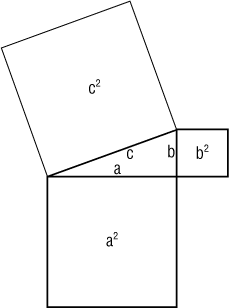
\includegraphics[width=50mm]{pythag}
\caption{Pythagoras' Theorem}
\label{fig:pythagoras}
\end{figure}
\end{lstlisting}
\caption{Including a Graphics File}\label{fig:lst:graphics}
\end{figure}

The result would be:

\begin{figure}[hbt!]\centering
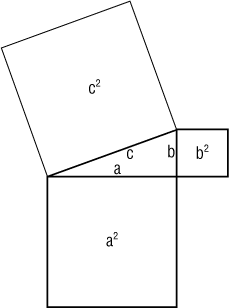
\includegraphics[width=50mm]{pythag}
\caption{Pythagoras' Theroem} \label{fig:pythagoras}
\end{figure}

Don't specify the extension of the graphic file.  The template will automatically look for the EPS or the PNG (or otherwise) versions, depending on whether \verb|latex| or \verb|pdflatex| was used.  The \texttt{figure} environment will also ensure that that an entry is inserted into the \emph{List of Figures} automatically -- including the figure numbering, caption and page number.

In addition, the width of the included graphics can also be specified as a percentage of the text width, e.g.~ \verb|width=.2\textwidth| would cause the graphics to occupy 20\% of the text width.

Notice that I inserted a \verb|\label| just after the \verb|\caption|.  This can be used for referencing the figure number, like this: \\
\verb|Figure \ref{fig:pythagoras}| $\to$ Figure \ref{fig:pythagoras}

This works the same for chapters, sections, tables, equations too.  In \verb|chap-intro.tex|, I labelled the Introduction chapter with \verb|\label{chap:intro}|.  I also labelled the section on inserting figures, \verb|\label{sec:figure}|.  So now I can do \\
\verb|Chapter \ref{chap:intro}| $\to$  Chapter \ref{chap:intro} \\
\verb|section \ref{sec:figure}| $\to$  section \ref{sec:figure}

Everytime the numbering of the heading changes, the reference will change automatically as well.  \textbf{This is another advantage of using \LaTeX{}}: you do not need to manually update the reference counters (nor the Table of Contents, List of Figures and Tables) whenever you add or remove figures, tables, sections or chapters.

You might also want to try out \texttt{Inkscape} or \texttt{FlowframTk}. Both program are a vector graphics and drawing application, and can export to \LaTeX{} code which you can paste into your \LaTeX{} source. \texttt{Inkscape} and \texttt{FlowframTk} are available from \url{https://inkscape.org/} and \url{https://www.dickimaw-books.com/software/flowframtk/}.

\section{How Do I Do Subfigures?}
Here's an example on how to do subfigures (and similarly subtables):

\begin{figure}[hbt!]
\begin{lstlisting}
\begin{figure}[hbt!]
  \begin{minipage}{.49\textwidth}
  \centering
  \subfloat[First caption]{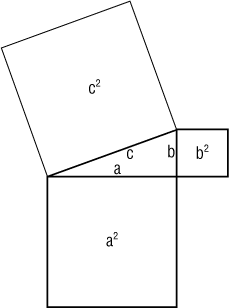
\includegraphics[width=3cm]{pythag}} \label{fig:sub1}
  \end{minipage}
  \hfill
  \begin{minipage}{.49\textwidth}
  \subfloat[Second caption]{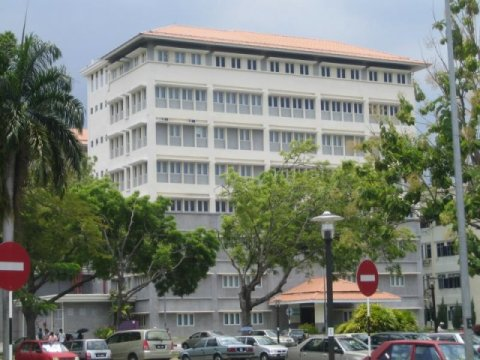
\includegraphics[width=0.8\textwidth]{USMScience}}\label{fig:sub2}
  \end{minipage}
  
  \caption{This is the main caption of the figure.}
  \label{fig:main}
\end{figure}
\end{lstlisting}
\caption{Creating subfigures within figures}
\end{figure}

\begin{figure}[hbt!]
  \begin{minipage}{.49\textwidth}
  \centering
  \subfloat[First caption]{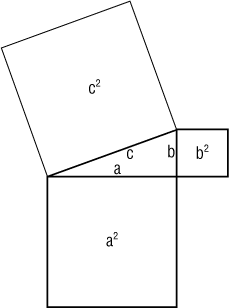
\includegraphics[width=3cm]{pythag}} \label{fig:sub1}
  \end{minipage}
  \hfill
  \begin{minipage}{.49\textwidth}
  \subfloat[Second caption]{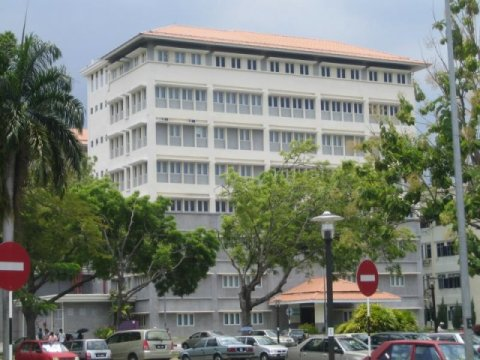
\includegraphics[width=0.8\textwidth]{USMScience}}\label{fig:sub2}
  \end{minipage}
  
  \caption{This is the main caption of the figure.}
  \label{fig:main}
\end{figure}

\section{Inserting Tables}

Typesetting tables can be a little troublesome especially with complex layouts.  Look up \citet{roberts} to learn about some tips, or you can use the online \LaTeX{} table generator (\url{https://www.tablesgenerator.com/}) to help you.

When you're done designing the table, copy the whole table as \LaTeX\ code, and paste it in your source file.  (You may add additional formatting commands, like bold, italics, etc.)  If this is going to be a numbered table, remember to surround it with \verb|\begin{table}| and \verb|\end{table}|, and give it a caption, like this:

\begin{figure}[hbt!]
\begin{lstlisting}
\begin{table}[hbt!]\centering
\begin{tabular}{| l | c || r |}
\hline
\textbf{Name} & \textbf{Category} & \textbf{Quantity} \\ 
\hline\hline
Apple & Fruit & 10 \\ 
\hline
Cucumber & Vegetable & 25 \\ 
\hline
Daisy & Flower & 5 \\ 
\hline
\end{tabular}
\caption{Sample Table Only} \label{table:sample}
\end{table}
\end{lstlisting}
\caption{Typesetting Tables}\label{fig:lst:table}
\end{figure}

\begin{table}[hbt!]\centering
\begin{tabular}{| l | c || r |}
\hline
\textbf{Name} & \textbf{Category} & \textbf{Quantity} \\ 
\hline\hline
Apple & Fruit & 10 \\ 
\hline
Cucumber & Vegetable & 25 \\ 
\hline
Daisy & Flower & 5 \\ 
\hline
\end{tabular}
\caption{Sample Table Only} \label{table:sample}
\end{table}

Note also that \verb|unimapcgsfyp| is configured such that captions for figures are placed \emph{below} the figures, and captions for tables are placed \emph{above} them, in accordance with the formatting guidelines.

Many of us would have had massive headaches about lining up decimal places in table columns if not for this tip from \citet[pp.~274--276]{latex:companion}. This method uses the \verb|dcolumn| package (already loaded by \verb|unimapcgsfyp.cls|). Instead of using \verb|L,C| or \verb|R| as the column type in the \verb|tabulary| declaration, use\\ \texttt{D\{\textit{input sep}\}\{\textit{output sep}\}\{\textit{decimal places}\}}. Note that in Table~\ref{tab:align:decimal}, I use \verb|tabulary| instead of \verb|tabular|. The \verb|tabulary| package is awesome. The column width is set automatically so that it will wrap long sentences into a few lines as demonstrated in Table~\ref{tab:tabletabulary}. 

\begin{figure}[htb!]
\begin{lstlisting}
\begin{table}[htb!]\centering
\begin{tabulary}{\textwidth}{| C | D{.}{.}{3} |}
\hline
Item & \multicolumn{1}{c|}{Reading}\\\hline
A & 1.11\\\hline
B & 3.99\\\hline
C & 2.27\\\hline
\end{tabulary}
\caption{A table with decimal data}
\end{table}
\end{lstlisting}
\caption{Aligning decimal data in tables}\label{fig:align:decimal}
\end{figure}

The \LaTeX\ code in Figure~\ref{fig:align:decimal} will give you Table~\ref{tab:align:decimal}.

\begin{table}[htb!]\centering
\begin{tabulary}{\textwidth}{| C | D{.}{.}{3} |}
\hline
Item & \multicolumn{1}{c|}{Reading}\\\hline
A & 1.11\\\hline
B & 3.999\\\hline
C & 22.2\\\hline
\end{tabulary}
\caption{A table with decimal data}\label{tab:align:decimal}
\end{table}

Without using \verb|dcolumn|, you'd get something like this:

\begin{table}[htb!]\centering
\begin{tabulary}{\textwidth}{| C | R |}
\hline
Item & \multicolumn{1}{c|}{Reading}\\\hline
A & 1.11\\\hline
B & 3.999\\\hline
C & 22.2\\\hline
\end{tabulary}
\caption{A table with decimal data (mis-aligned)}
\end{table}

\begin{table}[H]\singlespacing
	\caption{This is an example to for a table. This is straightforward version.}	\label{tab:tabletabulary}
	\begin{tabulary}{\textwidth}{L R C}
		\toprule[1.5pt]
		Short sentences & short one  & Long sentences \\ \midrule
		This is short.       & 173 & This is much loooooooonger, because there are many more words.  \\ 
		This is not shorter. & put some word here & This is still loooooooonger, because there are many more words. This table make use of \texttt{tabulary} package. \\ \bottomrule[1.5pt]
	\end{tabulary} 
\end{table}

In Table~\ref{tab:tabletabulary} and \ref{tab:tablemulticolumnrow}, I specify the position of the table as \verb|H| instead of \verb|tbh!| so that the table will appear \textbf{HERE} instead of giving the decision to \LaTeX\ for placing the table either \emph{top}, \emph{bottom}, or \emph{here}. 

\begin{figure}[tbh!]
	\begin{lstlisting}
		\begin{table}[H]\centering \singlespacing
		\caption{This is another example for a table. Advance version of a table.}	\label{tab:tablemulticolumnrow}
		\begin{tabulary}{0.8\textwidth}{|C|R|C|}
		\hline
		\multicolumn{2}{|c|}{\textbf{Merge 2 columns}} & \textbf{Long sentences} \\ \hline
		\multirow{2}{=}[-4.5mm]{This is short text LoL.} & \multicolumn{1}{c|}{\multirow{2}{*}{173}} & This is much loooooooonger, because there are many more words.  \\ \cline{2-3}
		& put some word here & This is still loooooooonger, because there are many more words. \\ \hline
		\end{tabulary} 
		\end{table} 
	\end{lstlisting}
	\caption{Note the differences between this table and previous tables.}
\end{figure}

\begin{table}[H]\centering \singlespacing
	\caption{This is another example for a table. Advance version of a table.}	\label{tab:tablemulticolumnrow}
	\begin{tabulary}{0.8\textwidth}{|C|R|C|}
		\hline
		\multicolumn{2}{|c|}{\textbf{Merge 2 columns}} & \textbf{Long sentences} \\ \hline
		\multirow{2}{=}[-4.5mm]{This is short text LoL.} & \multicolumn{1}{c|}{\multirow{2}{*}{173}} & This is much loooooooonger, because there are many more words.  \\ \cline{2-3}
		& put some word here & This is still loooooooonger, because there are many more words. \\ \hline
	\end{tabulary} 
\end{table} 

Table~\ref{tab:tablemulticolumnrow} set the table width so that it will occupy 80\% of the paper width. Then, I use \verb|multirow| package to span through 2 columns. This package also can be made to adjust the vertical alignment in a table whenever a row occupy more than a single line of sentence. \verb|multicolumn| not only use to merge two or more column, but can also be used to change a properties of a single row and column such as the text alignment and table border. 

\begin{table}[H]\centering\singlespacing
	\caption{This is an example to for a table}	\label{tab:tablemulticolumn}
	\begin{tabular}{|l|r|p{7cm}|}
		\hline
		\multicolumn{2}{|c|}{\textbf{Merge 2 columns}} & \textbf{Long sentences} \\ \hline
		\multirow{2}{*}[-4mm]{This is short.} & \multicolumn{1}{c|}{173} & This is much loooooooonger, because there are many more words.  \\ \cline{2-3}
		 & put some word here & This is still loooooooonger, because there are many more words. \\ \hline
	\end{tabular} 
\end{table} 

If you want to specify the exact size of each column, then make use of \verb|p{size}|, \verb|m{size}|, or \verb|b{size}|. \texttt{p} means normal cells, they are like parbox with alignment at the top line. \texttt{b} means alignment at the bottom, so the baseline is at the bottom line. \texttt{m} means alignment in the vertical center, i.e. the baseline is in the center. However, they not work very well with \verb|multitrow|. 

\section{Full-paged, Sideways Figures and Tables}

To make a figure appear on a landscape, full-page layout, put your \verb|\includegraphics| command in a \verb|sidewaysfigure| environment (Figure~\ref{fig:lst:sidewayfigure}).

\begin{figure}[htb!]
\begin{lstlisting}
\begin{sidewaysfigure}\centering
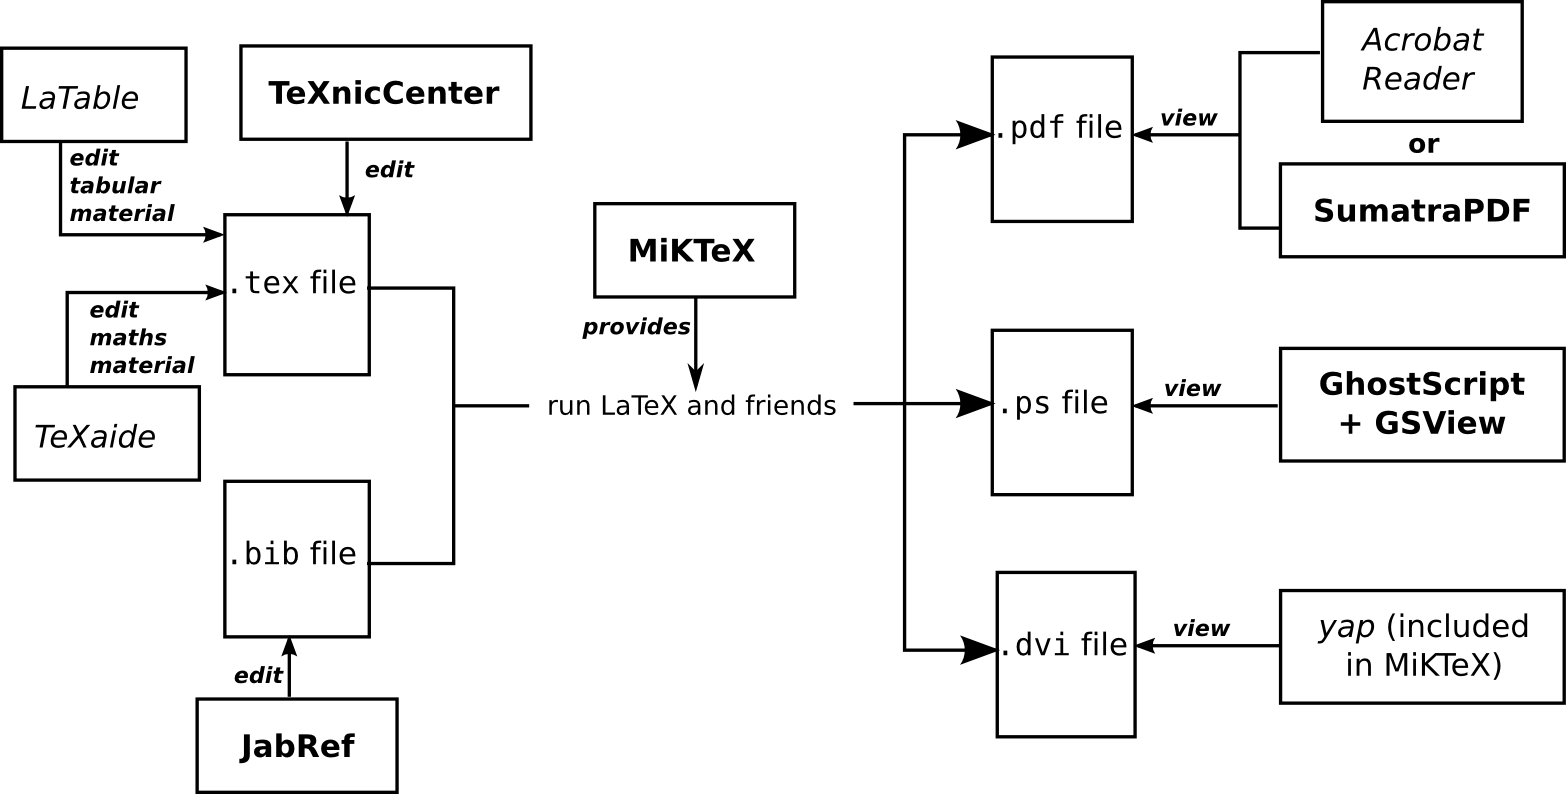
\includegraphics[width=\textheight]{latex-win-comp}
\caption{A full-page, sideways figure}\label{fig:sidewaysfig}
\end{sidewaysfigure}
\end{lstlisting}
\caption{Including a sideway, full-page graphic}\label{fig:lst:sidewayfigure}
\end{figure}

\begin{sidewaysfigure}
\centering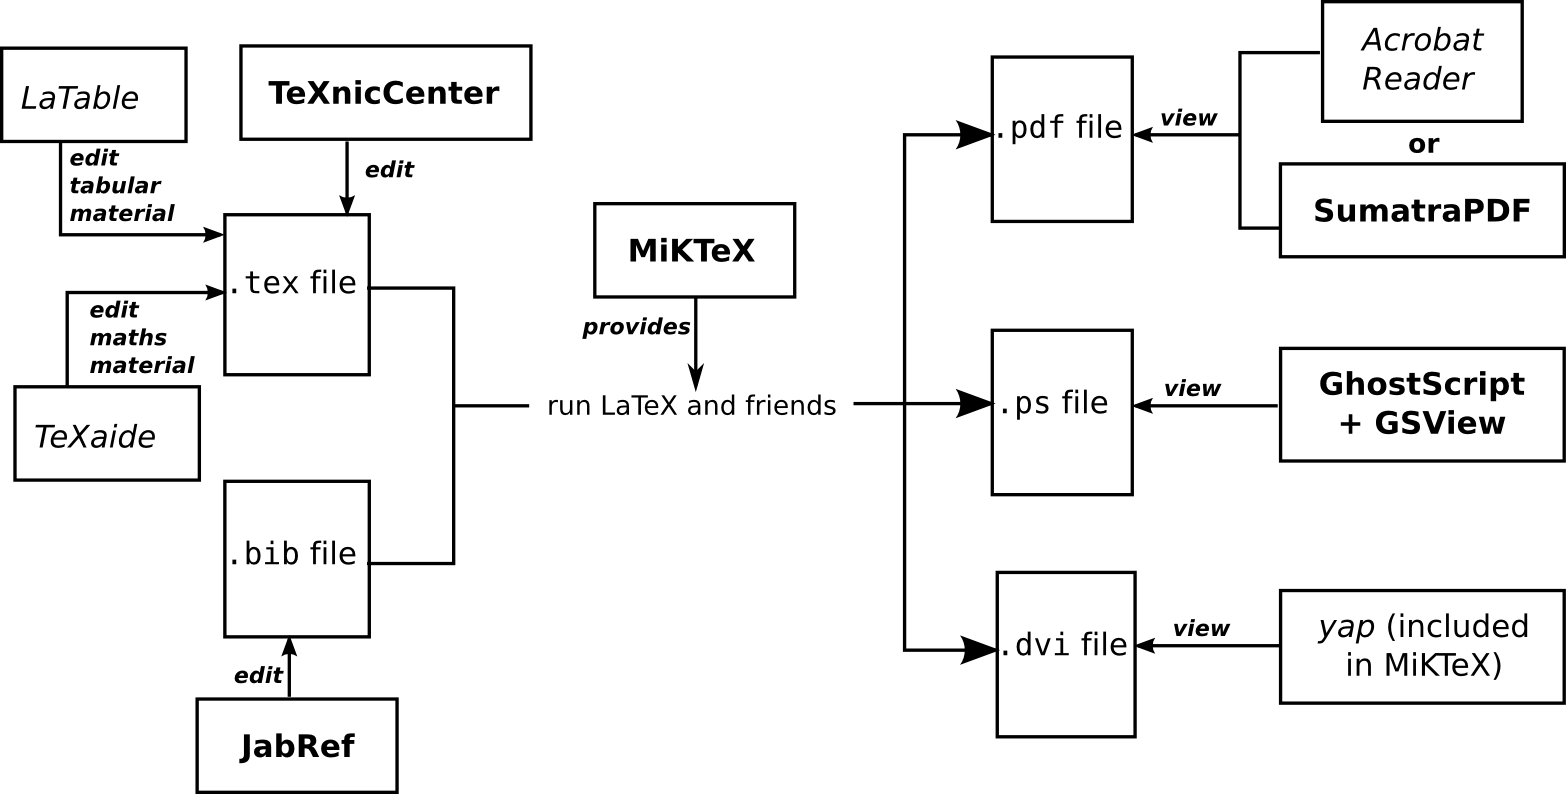
\includegraphics[width=\textheight]{latex-win-comp}
\caption{A full-page, sideways figure}\label{fig:sidewaysfig}
\end{sidewaysfigure}

The resultant figure (Figure~\ref{fig:sidewaysfig}) should appear on the next page.

\begingroup
\setlength{\rotFPtop}{1pc} %
\begin{sidewaystable}
	\singlespacing
		\caption{This is an example to for a table. This is straightforward version.}	\label{tab:sidetabletabulary}
		\begin{tabulary}{\textwidth}{L R C}
			\toprule[1.5pt]
			Short sentences & short one  & Long sentences \\ \midrule
			This is short.       & 173 & This is much loooooooonger, because there are many more words.  \\ 
			This is not shorter. & put some word here & This is still loooooooonger, because there are many more words. This table make use of \texttt{tabulary} package. \\ \bottomrule[1.5pt]
		\end{tabulary} 
\end{sidewaystable}
\endgroup

For a sideways table, use the \verb|sidewaystable| environment instead around your usual \verb|tabular| material. The default positioning of the figure/table is in the middle of a page. You can use \verb|\setlength{\rotFPtop}{1pc}| before the \verb|sidewaystable| environment to change the figure/table positioning. Please enclose the \verb|sidewaystable| environment inside \verb|begingroup| and \verb|endgroup| so that it won't affect the positioning of the figure/table of the whole document. Play around with the size, 1pc, 0pt etc. 

\section{Mathematical Equations}

%Oooh I love this one.  After all, maths is the reason why Donald Knuth created \TeX{}!  It would be quite impossible for me to list all the commands, so I'll just give some example here, and you're better off looking at the various online tutorials like \cite{roberts}.  And TeXnicCenter certainly makes things much easier.

Typesetting mathematical material is one of, if not \emph{the}, strongest capabilities of \LaTeX.  After all, that was the Knuth's main motivation for creating \TeX{}.  As it is impossible to enumerate all possible mathematically-related commands and macros here, we will just give some examples.  The reader is directed to the many well-written online tutorials, such as \citet{roberts}, for more elaborate examples.  TeXnicCenter also provides many shortcut buttons for inserting mathematical symbols.

\begin{figure}[htb!]
\begin{lstlisting}
\begin{equation}\label{eq:pythagoras}
z^2 = x^2 + y^2
\end{equation}

\begin{equation}\label{eq:golden:ratio}
\phi = \frac{1}{2} (1 + \sqrt{5})
\end{equation}

\begin{equation}\label{eq:golden:ratio}
\phi = \frac{1}{2} (1 + \sqrt{5})
\end{equation}
\begin{equation}\label{eq:golden:ratio:fibonacci}
\phi = 1 + \sum ^ {\infty} _ {n=1}
                \frac{ (-1) ^ {n+1} }{ F_n F_{n+1} }
\end{equation}

Equation~\ref{eq:pythagoras} is the Pythagoras Theorem. 
\eqref{eq:golden:ratio} gives the golden ratio $\phi$, and 
\eqref{eq:golden:ratio:fibonacci} relates it to the Fibonacci 
series.
\end{lstlisting}
\caption{Typesetting Mathematical Equations}\label{fig:lst:equation}
\end{figure}

\begin{equation}\label{eq:pythagoras}
z^2 = x^2 + y^2
\end{equation}
\begin{equation}\label{eq:golden:ratio}
\phi = \frac{1}{2} (1 + \sqrt{5})
\end{equation}
\begin{equation}\label{eq:golden:ratio:fibonacci}
\phi = 1 + \sum ^ {\infty} _ {n=1}
                \frac{ (-1) ^ {n+1} }{ F_n F_{n+1} }
\end{equation}

Equation~\ref{eq:pythagoras} is the Pythagoras Theorem. \eqref{eq:golden:ratio} gives the golden ratio $\phi$, and \eqref{eq:golden:ratio:fibonacci} relates it to the Fibonacci series.

The \LaTeX\ code to generate the above mathematics materials are shown in Figure~\ref{fig:lst:equation}.  As you can see, references to equations can be achieved with either \verb|\ref| or \verb|\eqref|. 

You might want to try the online equation edit \url{https://www.mathcha.io/} or \url{https://www.latex4technics.com/} to familiarize with the \LaTeX\ equation. 

\section{Acronyms}
\acresetall
If you have a list of acronyms or symbols, edit the file \verb|loa.tex| as in Figure~\ref{fig:acronym}.

\begin{figure}[hbt!]
\begin{lstlisting}
\begin{acronym}[MMMMMM] %% replace 'MMMMMM' with the longest acronym in your list
\acro{CGS}{Centre for Graduate Studies}
\acro{PPKMt}{Pusat Pengajian Kejuruteraan Mekatronik}
\acro{USM}{Universiti Sains Malaysia}
\acro{UniMAP}{Universiti Malaysia Perlis}
\end{acronym}
\end{lstlisting}
\caption{The template \texttt{loa.tex} for acronyms}\label{fig:acronym}
\end{figure}

You can also use this acronym list to help expand it the first time you mention it in your text.  For example, the first time you use \verb|\ac{UniMAP}|, `\ac{UniMAP}' will be the output (without the quotes).  After that, all calls to \verb|\ac{UniMAP}| will give `\ac{UniMAP}' (without the quotes).  For more information, see the documentation for the \texttt{acronym} package.

\section{Program Listings}

You may have noticed that I used the \verb|lstlisting| environment to typeset some of the \LaTeX{} examples -- with pretty-printing\footnote{Whether you agree that it \emph{is} pretty is another story altogether.}, too, including automatic line-breaking.  For more information, see the documentation for the \verb|listings| package: it's available online at \url{http://www.texdoc.net/pkg/listings}.

Just to give some simple example here.  For example, to typeset a ``Hello World'' Java program with syntax highlighting, you can use the following code:

\begin{figure}[hbt!]
\begin{lstlisting}[escapechar=:,language={}]
\lstset{basicstyle=\small\ttfamily, language=Java, breaklines=true, columns=fullflexible, tabsize=2}
\begin{lstlisting}
public class HelloWorld {
	public static void main( String arg[] ) {
        for (int i = 0; i < 10; i++) {
			System.out.println( "Hello World!" + i);
		}
	}
}
\end:\{:lstlisting:\}:
\end{lstlisting}
\caption{Typesetting a Java program listing}\label{fig:lst:syntax}
\end{figure}

\lstset{keywordstyle={\bfseries}}
\begin{figure}[hbt!]
\lstset{basicstyle=\small\ttfamily, language=Java, breaklines=true, columns=fullflexible, framesep=10pt, xleftmargin=16pt, tabsize=2}
\begin{lstlisting}
public class HelloWorld {
	public static void main( String arg[] ) {
        for (int i = 0; i < 10; i++) {
			System.out.println( "Hello World!" + i);
		}
	}
}
\end{lstlisting}
\caption{A pretty-printed Java program listing with syntax highlighting}
\end{figure}


If you want to turn off the syntax highlighting, set \verb|language={}|.  (See the \verb|listings| documentation for a list of programming languages for which syntax highlighting is supported.)  You can also change the \verb|basicstyle| value to get different effects: e.g. a different font family, size or text formatting.

Here's another example for a C program:

\begin{figure}[hbt!]
\begin{lstlisting}[escapechar={:}, texcl=false,language={}]
\lstset{basicstyle=\sffamily, language=C, breaklines=true, columns=fullflexible, tabsize=2}
\begin{lstlisting}
int main() {
	int c = 0;
	c = c + 1;
	printf( "%d", c );
	return 0;
}
\end:\{:lstlisting:\}:
\end{lstlisting}
\caption{Typesetting a C program listing}\label{fig:lst:c}
\end{figure}

\begin{figure}[hbt!]
\lstset{basicstyle=\sffamily, language=C, breaklines=true, columns=fullflexible, framesep=10pt, xleftmargin=.4\textwidth, tabsize=4}
\begin{lstlisting}
int main() {
	int c = 0;
	c = c + 1;
	printf( "%d", c );
	return 0;
}
\end{lstlisting}
\caption{A pretty-printed C program listing with syntax highlighting}
\end{figure}


And here is the same C program listing \emph{without} syntax highlighting (by setting \verb|language={}|):

\begin{figure}[H]

\lstset{basicstyle=\sffamily, language={}, breaklines=true, columns=fullflexible, framesep=10pt, xleftmargin=.4\textwidth, tabsize=4}
\begin{lstlisting}
int main() {
	int c = 0;
	c = c + 1;
	printf( "%d", c );
	return 0;
}
\end{lstlisting}
\caption{A C program listing without syntax highlighting}
\end{figure}
